\documentclass[10pt, aspectratio=169]{beamer}
\usepackage{minted}
\usepackage[T2A]{fontenc}
\usepackage{graphicx} % Required for inserting images
\usepackage{tikz}
\usetikzlibrary{patterns}
%\usepackage[russian]{babel} % Поддержка русского языка
%\setbeamerfont{institute}{size=\normalsize}

\title{Научно-исследовательская практика. Cryptohack: Lack of Entropy (Firebird Internal CTF)}
\author{Винников Кирилл, Затирахин Кирилл }
\date{Июль 2023}

\usetheme{Antibes}

\begin{document}

\maketitle

\begin{frame}[fragile]{Условие задачи}
    Дана программа, шифрующая исходное сообщение с помощью алгоритма RSA. Также дан файл с выводом представленной программы. Конкретно: модуль по которому ведутся вычисления \textbf{\emph{n}}, экспонента шифрования \textbf{\emph{e}}, зашифрованное сообщение \textbf{\emph{c}} Необходимо расшифровать исходное сообщение.

    Ниже представлен фрагмент исходного кода задачи, где генерируются простые \textbf{\emph{p}} и \textbf{\emph{q}}

    \begin{minted}[frame=single,framesep=3pt]{python}
        #e = 65537
        while True:
            p = random.getrandbits(256)
            q = int(gmpy2.digits(p, 3))
            # Ensure that they are prime
            if not gmpy2.is_prime(p): continue
            if not gmpy2.is_prime(q): continue
            # Ensure that d exists
            if (p-1) % e == 0: continue
            if (q-1) % e == 0: continue
            break
    \end{minted}
    
\end{frame}

\begin{frame}[fragile]{Метод решения}
    Число \textbf{\emph{n}} зависит от простых чисел \textbf{\emph{p}} и \textbf{\emph{q}}. В свою очередь, число \textbf{\emph{q}} напрямую зависит от \textbf{\emph{p}}. Число \textbf{\emph{p}} генерируется длиной 256 бит, то оно находится в промежутке от $2^{255}$ до $2^{256}$. \\\\Таким образом, задача сводится к поиску такого простого числа \textbf{\emph{p}}, что полученный модуль совпадет с исходным. Если это произойдет, можно легко вычислить функцию Эйлера $\varphi$ и найти обратный эелемент по отношению к экспоненте \textbf{\emph{e}} и расшифровать сообщение.
\end{frame}

\begin{frame}{Визуализация}
\centering
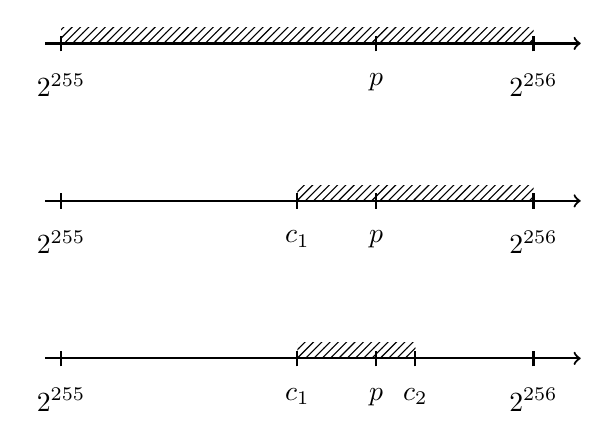
\begin{tikzpicture}[mydrawstyle/.style={draw=black, thick}, x=1mm, y=1mm, z=1mm]
  \draw[mydrawstyle, ->](-2,50)--(66,50);
  \draw[mydrawstyle](0,49)--(0,51) node[below=10]{$2^{255}$};
  \draw[mydrawstyle](40,49)--(40,51) node[below=10]{$p$};
  \draw[mydrawstyle](60,49)--(60,51) node[below=10]{$2^{256}$};
  \fill[pattern=north east lines] (0,52) rectangle (60,50);

  \draw[mydrawstyle, ->](-2,30)--(66,30);
  \draw[mydrawstyle](0,29)--(0,31) node[below=10]{$2^{255}$};
  \draw[mydrawstyle](30,29)--(30,31) node[below=10]{$c_1$};
  \draw[mydrawstyle](40,29)--(40,31) node[below=10]{$p$};
  \draw[mydrawstyle](60,29)--(60,31) node[below=10]{$2^{256}$};
  \fill[pattern=north east lines] (30,32) rectangle (60,30);

  \draw[mydrawstyle, ->](-2,10)--(66,10);
  \draw[mydrawstyle](0,9)--(0,11) node[below=10]{$2^{255}$};
  \draw[mydrawstyle](30,9)--(30,11) node[below=10]{$c_1$};
  \draw[mydrawstyle](45,9)--(45,11) node[below=10]{$c_2$};
  \draw[mydrawstyle](40,9)--(40,11) node[below=10]{$p$};
  \draw[mydrawstyle](60,9)--(60,11) node[below=10]{$2^{256}$};
  \fill[pattern=north east lines] (30,12) rectangle (45,10);
\end{tikzpicture}
    
\end{frame}

\begin{frame}[fragile]{Решение (фрагмент кода)}
    \begin{minted}[frame=single,framesep=3pt]{python}
        first = gmpy2.next_prime(2**255)
        last = gmpy2.next_prime(2**256)
        p = -1
        q = -1
        while (first <= last) and (p == -1):
            p0 = gmpy2.next_prime((first+last)//2)
            q0 = int(gmpy2.digits(p0, 3))
            N=p0*q0
            if (N == n):
                p = p0
                q = q0
            else:
                if (N<n):
                    first = p0 +1
                else:
                    last = p0 -1
    \end{minted}
\end{frame}

\begin{frame}{Вывод и проверка результата}
    \begin{figure}[h]
    \centering
    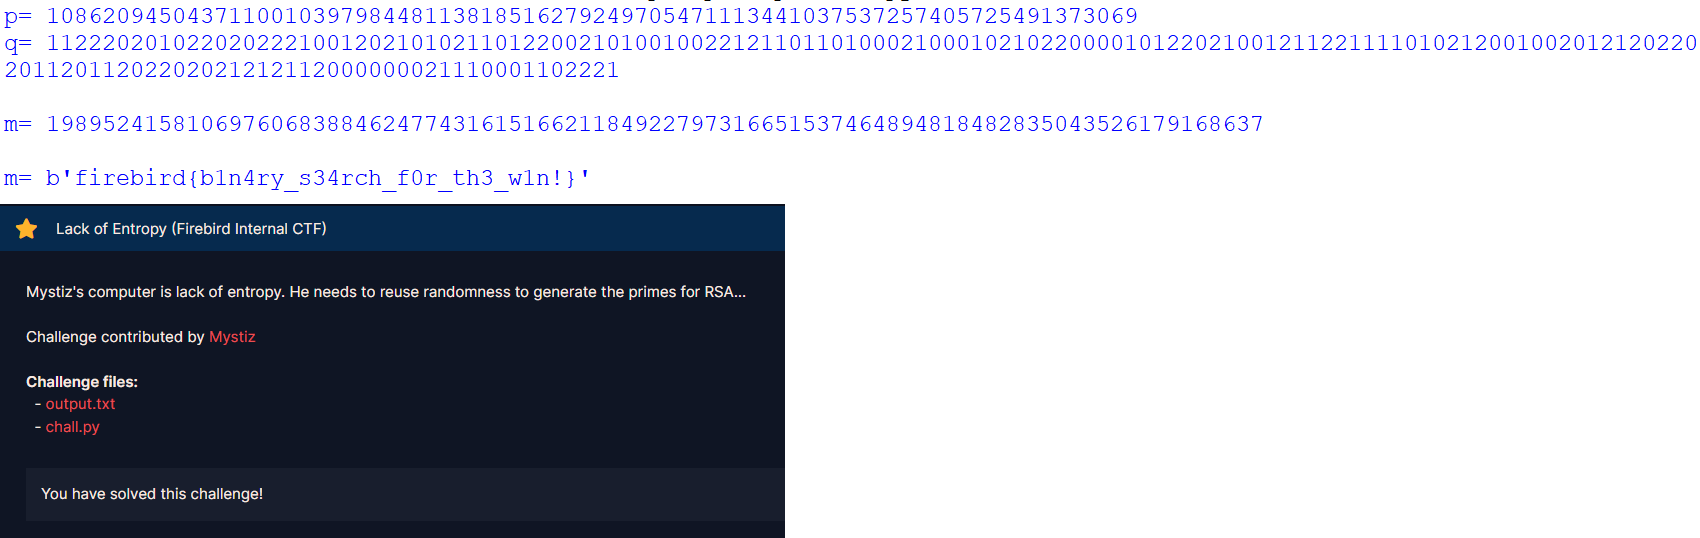
\includegraphics[width=1\linewidth]{123123123.png}
    \label{fig:mpr}
    \end{figure}
\end{frame}

\end{document}
